\chapter{Synthesizing a Verilog Module}
\graphicspath{ {./Lab00HowTo/howTo40 Performing Synthesis/Fig} }

The combinedLab01 verilog file used in this example has three inputs and
three outputs that are mapped to slide switches and LEDs.

It's time to realize the \emph{combinedLab01} Verilog file to FPGA. To
do this follow these steps:

\begin{enumerate}
\def\labelenumi{\arabic{enumi}.}
\item
  In Project Navigator pane, select the File tab
\item
  Right mouse click \emph{combinedLab01.v} and select Set As Top Level
  Entity.
\item
  Processing -\textgreater{} Start -\textgreater{} Start Analysis and
  Elaboration
\item
  Assignments -\textgreater{} Pin Planner
\item
  In the Pin Planner pop-up you should see the pin assignment pane at
  the bottom of the window.

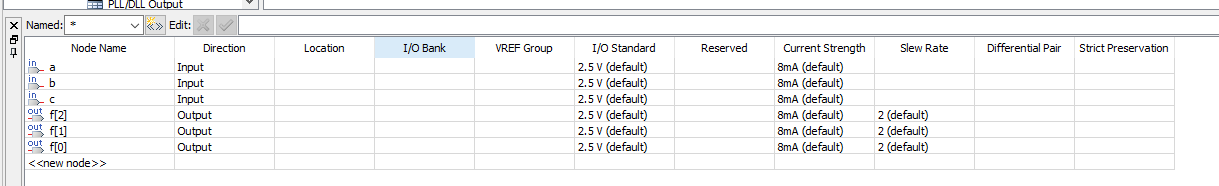
\includegraphics{image1.png}

\item
  Double click in the Location cell for row c
\item
  Scroll down the list of pins to PIN\_AC9
\item
  Complete the pin assignment for the other 5 inputs and outputs using
  the information contained in pin assignment table completed earlier.
\item
  Double check your pin assignments.
\item
  File -\textgreater{} Close. Note closing your file incorporates this
  assignment into the project.
\item
  Back in the Quartus window, Processing -\textgreater{} Start
  Compilation \textless Ctrl-L\textgreater{}
\item
  Tools -\textgreater{} Programmer
\item
  In the Programmer pop-up window click Add File\ldots{}
\item
  In the Select Programming File pop-up, navigate to your project
  directory, then into the output files folder, the select
  combinedLab01.sof, click Open. You should see something like the
  following.

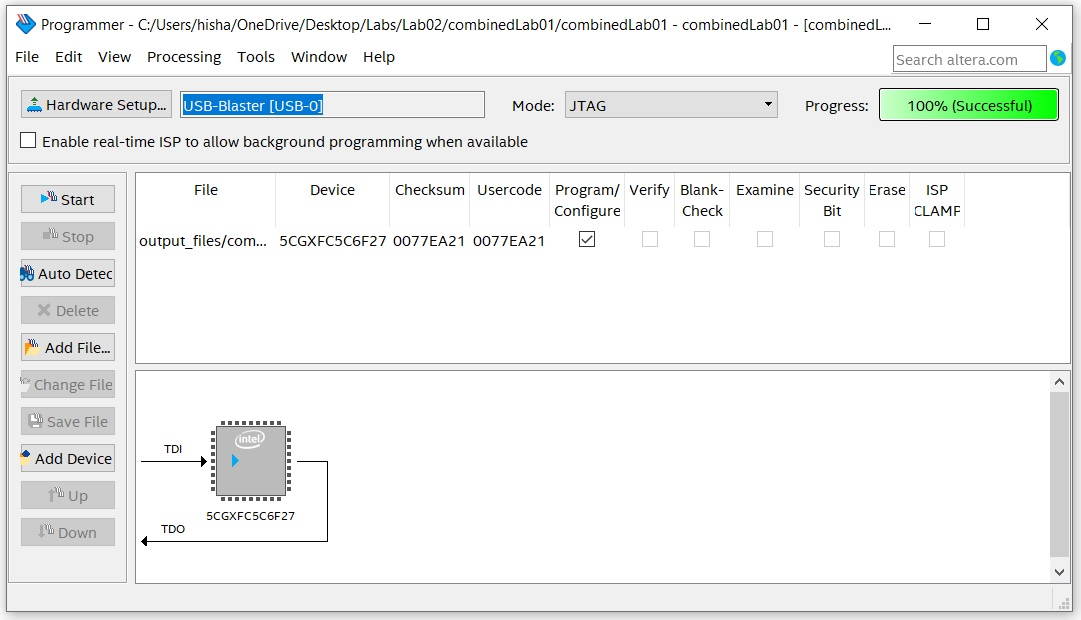
\includegraphics{image2.png}

\item
  Connect the Altera Cyclone V GX FPGA to your computer through the USB
  port, connect the power supply, and push the red power-on button. Try
  not to be annoyed by the infernal blinking LEDs.
\item
  In the Programmer pop-up

  \begin{enumerate}
  \def\labelenumii{\alph{enumii}.}
  \item
    Click Hardware Setup\ldots.
  \item
    In the Hardware Setup select USB-Blaster {[}USB=0{]} from the
    Currently selected hardware pull-down
  \item
    Click Close
  \end{enumerate}
\item
  Back in the Programmer window, the box next to Hardware Setup\ldots{}
  should reflect your choice. Click Start,
\item
  The Development board should stop its infernal blinking and run your
  program. Your design is now running on the FPGA.
\end{enumerate}


